\chapter{Architecture Design}
\label{kap:architecture_design}

In this chapter, we present architecture for all models that we decided to train, specifically \textbf{EnvMap} for estimating environment maps, \textbf{IRN} for estimating intrinsic properties, \textbf{RAR} for indirect illumination  and \textbf{MSN} for material segmentation. Our whole pipeline for inverse rendering and material segmentation is shown in figure \ref{img:architecture}.
\begin{figure}[H]
    \centerline{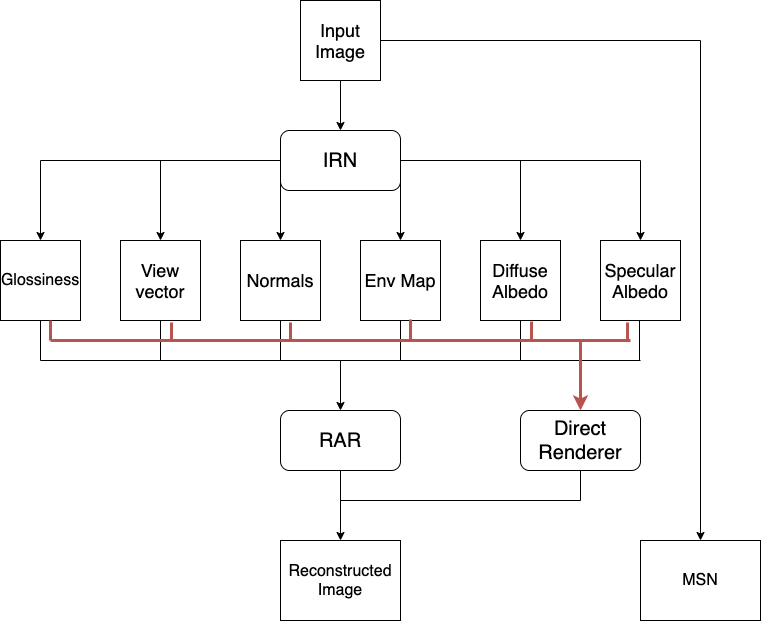
\includegraphics[width=0.6\textwidth]{praca/images/MaterialPicker-network-architecture.png}}
    \caption[Our pipeline]{Our pipeline}
    \label{img:architecture}
\end{figure}
\section{EnvMap}
\label{sec:env-map-architecture}
Our EnvMap model's architecture is defined as follows:
\newline

ReflectionPad(3) $\to$ Conv7$\times$7(3, 64) $\to$ Conv3$\times$3(64, 128) $\to$

Conv3$\times$3(128, 256) $\to$ 4 $\times$ ResNetBlock(256) $\to$ Conv1$\times$1(256, 256) $\to$ 

Conv3$\times$3(256, 256) $\to$ Conv3$\times$3(256, 128) $\to$ Conv3$\times$3Tanh(128, 3) $\to$ 

Upsample(18, 36)
\newline
\newline
where ConvN$\times$N($x, y$) indicate 2D convolutional layer with kernel of size $N \times N$ and stride 2, $x$ input channels and $y$ output channels, succeeded by batch normalization and ReLU activation; ConvN$\times$NTanh($x, y$) stands for ConvN$\times$N($x, y$), but with Tanh as activation function; ReflectionPad(N) represents reflection padding with N padded items in each direction; Upsample($x, y$) denotes layer that upsamples input into output with size $x \times y$ using bilinear interpolation and 4 $\times$ ResNetBlock(N) is a series of 4 consecutive block, with each ResNetBlock being
\newline

ReflectionPad(1) $\to$ Conv3$\times$3(N, N) $\to$ BN(N) $\to$
ReLU $\to$

ReflectionPad(1) $\to$ Conv3$\times$3(N, N) $\to$ BN(N)
\newline
\newline
where BN(N) denotes batch normalization over input of size N $\times$ N.
\section{IRN}
\label{sec:irn-architecture}
IRN consists of encoder \textbf{Enc}, defined as 
\newline

ReflectionPad(3) $\to$ Conv7x7(3, 64) $\to$ Conv3x3(64, 128) $\to$ Conv3x3(128, 256)
\newline
\newline
which output is then fed through 9 $\times$ ResNetBlock for each estimated parameter except for light estimation, which is handled separately. Each parameter (except for light) is then upsampled to original input size by decoder \textbf{Dec}, defined as
\newline
 
TransConv3$\times$3(256, 128) $\to$ TransdConv3$\times$3(128, 64) $\to$ ReflectionPad(3) $\to$

Conv7$\times$7(64, 3) $\to$ Tanh
\newline
\newline
with glossinness as an exception, which the second-to-last layer is  Conv7$\times$7(64, 1). TransConvN$\times$N($x, y$) represent transposed convolution with kernel size N $\times$ N, $x$ input and $y$ output feature maps respectively.
\newline
Input to light estimation module is concatenation of \textbf{Enc} output and output after 9 $\times$ ResNetBlocks for every estimated parameter along channel dimension, which yields
\newline

Conv1$\times$1(1536, 256), $\to$ Conv3$\times$3(256, 256), $\to$ Conv3$\times$3(256, 128), $\to$

Conv3$\times$3Tanh(128, 3), $\to$ Upsample((18, 36))

\section{RAR}
\label{sec:rar-architecture}
RAR architecture is implemented in encoder-decoder fashion, which is taken from U-Net \cite{u-net}, alongside encoder for the input image.
Encoder for the input image is defined as
\newline

ReflectionPad(3) $\to$ Conv7$\times$7(3, 64) $\to$ Conv3$\times$3(64, 128) $\to$

Conv3$\times$3(128, 256) $\to$ Conv1$\times$1(256, 128) Conv3$\times$3S1(128, 64) $\to$

Conv3$\times$3(64, 32) $\to$ Conv3$\times$3(32, 16) $\to$ Linear(4800, 300)
\newline
\newline
with transformation between output of second-last layer of spatial resolution (16 $\times$ 15 $\times$ 20) into 4800 features as input into the last linear layer; ConvN$\times$NS1($x, y$) denotes the same as ConvN$\times$N($x, y$), but with stride 1.
\newline
U-net encoder \textbf{Enc} takes all estimated parameters, concatenated along channel dimension 
\newline

Conv3$\times$3S1(13, 64) $\to$ Conv3$\times$3(64, 64) $\to$ Conv3$\times$3(64, 128) $\to$

Conv3$\times$3(128, 256) $\to$ Conv3$\times$3(256, 512)
\newline
\newline
and decoder \textbf{Dec} specified as
\newline

UpConv3$\times$3(513, 512) $\to$ UpConv3$\times$3(768, 256) $\to$ UpConv3$\times$3(384, 128) $\to$

UpConv3$\times$3(192, 64) $\to$ Conv1$\times$1Tanh(64, 3)
\newline
\newline
where UpConvN$\times$N($x, y$) is block defined as
\newline

Upsample(2) $\to$ Convolution3$\times$3P1($x, y$) $\to$ BN($y$) $\to$ ReLU.
\newline
\newline
where Upsample(2) is layer that upsamples input by factor of 2 and Conv3$\times$3P1($x, y$) denotes 2D convolutional layer with kernel of size 3$\times$3, $x$ input a $y$ output channels, stride 2 and padding 1.
Skip connections are implemented between Conv3$\times$3(*, N) and UpConv3$\times$3(*, N).
\section{MSN}
\label{sec:msn-architecture}
Architecture for MSN is set as \;\; \textbf{Enc} $\to$ 9 $\times$ ResNetBlock $\to$ \textbf{Dec} \;\;
with ResnetBlock defined in section \ref{sec:env-map-architecture} and \textbf{Enc} and \textbf{Dec} defined in section \ref{sec:irn-architecture}.